\documentclass[aspectratio=43,english]{beamer} %If you want to create Polish presentation, replace 'english' with 'polish' and uncomment 3-th line, i.e., '\usepackage{polski}'
\usepackage[utf8]{inputenc}
\usepackage{polski} %Uncomment for Polish language
\usepackage{babel}
\usepackage{listings} %We want to put listings

\mode<beamer>{ 	%in 'beamer' mode
	\hypersetup{pdfpagemode=FullScreen}		%Enable Full screen mode
	\usetheme{JuanLesPins} 		%Show part title in right footer
	%\usetheme[dark]{AGH}                 		%Use dark background
	%\usetheme[dark,parttitle=leftfooter]{AGH}  	%Use dark background and show part title in left footer
}
\mode<handout>{	%in 'handout' mode
	\hypersetup{pdfpagemode=None}		
	\usepackage{pgfpages}
  	\pgfpagesuselayout{4 on 1}[a4paper,border shrink=5mm,landscape]	%show 4 slides on 1 page
  	\usetheme{boxes}
  	\addheadbox{structure}{\quad\insertpart\hfill\insertsection\hfill\insertsubsection\qquad} 	%content of header
 	\addfootbox{structure}{\quad\insertauthor\hfill\insertframenumber\hfill\insertsubtitle\qquad} 	%content of footer
}

\AtBeginPart{ %At begin part: display its name
	\frame{\partpage}
} 


%%%%%%%%%%% Configuration of the listings package %%%%%%%%%%%%%%%%%%%%%%%%%%
% Source: https://en.wikibooks.org/wiki/LaTeX/Source_Code_Listings#Using_the_listings_package
%%%%%%%%%%%%%%%%%%%%%%%%%%%%%%%%%%%%%%%%%%%%%%%%%%%%%%%%%%%%%%%%%%%%%%%%%%%%
\lstset{ %
  backgroundcolor=\color{white},   % choose the background color
  basicstyle=\footnotesize,        % the size of the fonts that are used for the code
  breakatwhitespace=false,         % sets if automatic breaks should only happen at whitespace
  breaklines=true,                 % sets automatic line breaking
  captionpos=b,                    % sets the caption-position to bottom
  commentstyle=\color{green},      % comment style
  deletekeywords={...},            % if you want to delete keywords from the given language
  escapeinside={\%*}{*)},          % if you want to add LaTeX within your code
  extendedchars=true,              % lets you use non-ASCII characters; for 8-bits encodings only, does not work with UTF-8
  frame=single,	                   % adds a frame around the code
  keepspaces=true,                 % keeps spaces in text, useful for keeping indentation of code (possibly needs columns=flexible)
  keywordstyle=\color{blue},       % keyword style
  morekeywords={*,...},            % if you want to add more keywords to the set
  numbers=left,                    % where to put the line-numbers; possible values are (none, left, right)
  numbersep=5pt,                   % how far the line-numbers are from the code
  numberstyle=\tiny\color{gray},   % the style that is used for the line-numbers
  rulecolor=\color{black},         % if not set, the frame-color may be changed on line-breaks within not-black text (e.g. comments (green here))
  showspaces=false,                % show spaces everywhere adding particular underscores; it overrides 'showstringspaces'
  showstringspaces=false,          % underline spaces within strings only
  showtabs=false,                  % show tabs within strings adding particular underscores
  stepnumber=2,                    % the step between two line-numbers. If it's 1, each line will be numbered
  stringstyle=\color{cyan},        % string literal style
  tabsize=2,	                   % sets default tabsize to 2 spaces
  title=\lstname,                  % show the filename of files included with \lstinputlisting; also try caption instead of title
                                   % needed if you want to use UTF-8 Polish chars
  literate={?}{{\k{a}}}1
           {?}{{\k{A}}}1
           {?}{{\k{e}}}1
           {?}{{\k{E}}}1
           {�}{{\'o}}1
           {�}{{\'O}}1
           {?}{{\'s}}1
           {?}{{\'S}}1
           {?}{{\l{}}}1
           {?}{{\L{}}}1
           {?}{{\.z}}1
           {?}{{\.Z}}1
           {?}{{\'z}}1
           {?}{{\'Z}}1
           {?}{{\'c}}1
           {?}{{\'C}}1
           {?}{{\'n}}1
           {?}{{\'N}}1
}
%%%%%%%%%%%%%%%%%


\title{Metody Obliczeniowe w Nauce i Technice}
\author{Marian Bubak, PhD}
\date{}
\institute[AGH]{
	Institute of Computer Science\\ul. Kawiory 21\\30-055 Krakow\\
	Poland\\
	\url{http://www.icsr.agh.edu.pl/~mownit/}
}


\usepackage{amsmath}
\usepackage{mathtools}
\subtitle{6 - Kwadratury - całkowanie numeryczne}
\begin{document}
  	\maketitle
	%%%%%%%%%%%%%%%%
	\begin{frame}{Outline}
		\tableofcontents
	\end{frame}
	%%%%%%%%%%%%%%%%
	\section{Wstęp}
%%%%%%%%%%%%%%%%%%%%%%%%%
	\begin{frame}{Wstęp} 
		\textcolor{blue}{Problem:}

		\begin{itemize}
			\item Wiele całek nieoznaczonych nie daje się wyrazić w postaci skończonej przez funkcje elementarne
			\item Częsta niemożliwość znalezienia dokładnych całek oznaczonych
    	\end{itemize}

		\textcolor{blue}{Przykłady:}
		\begin{itemize}
			\item $\int_{0}^{2}e^{-x^{2}} dx$
			\item $\int_{0}^{\pi}cos(3cos\theta) d\theta$
    	\end{itemize}
    	
    	\textcolor{blue}{Rozwiązanie:}
    	\begin{itemize}
    	\item Zastąpienie funkcji podcałkowej $f(x)$ inną bliską funkcją $g(x)$, przybliżenie całki przez sumę ważoną:
    	\end{itemize}
    	$$I=\int_{a}^{b}f(x)dx \approx\sum_{i=0}^{n}A_{i}y_{i}$$
   	 	
	\end{frame}
%%%%%%%%%%%%%%%%%%%%%%%%%
	\begin{frame}
    
a) \textit {kwadratura} - przypadek specjalny zagadnienia początkowego\footnote{zagadnienie polegające na znalezieniu konkretnej funkcji spełniającej dane równanie różniczkowe i warunek początkowy.}:
$$
 I=\int_{a}^{b}f(x)dx\ \equiv I=y(b)
$$
\textcolor{blue}{Dane:} 
\begin{itemize}
	\item pochodna: $\displaystyle \frac{dy}{dx}=f(x)$
	\item warunek początkowy: $(a)=0$
  \end{itemize}
\end{frame}
%%%%%%%%%%%%%%%%%%%%%%%%%	    
    \begin{frame}
    
      b)
      \begin{center}
      	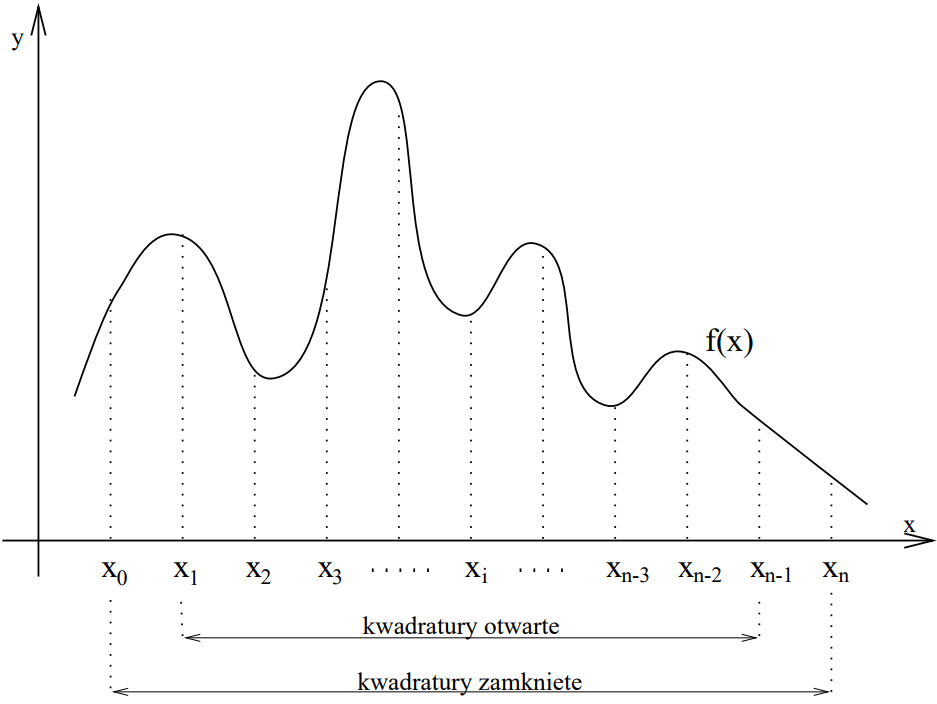
\includegraphics[width=0.6\linewidth]{img/6/image001.png}
      \end{center}
      
      \begin{block}{}
      Kwadratury:
      
        \begin{itemize}
          \item otwarte 
          \item zamknięte
          \item półotwarte
        \end{itemize}
      \end{block}
    \end{frame}
%%%%%%%%%%%%%%%%%%%%%%%%%
    \begin{frame}
    	c) \textbf{Istota}: $\newline$
    	 Podział przedziału całkowania [a,b] na podprzedziały $\rightarrow$ formuły złożone
        $$
	        I=\int_{a}^{b}f(x)dx\ = \sum_{i=0}^{n}\int_{a_{i}}^{a_{i+1}}f(x)dx=\sum_{i=0}^{n}I_{i}
        $$
		d) \textbf{Stopień dokładności kwadratury}: $\newline$
        \textit{E} - błąd kwadratury,$\newline$
         {$P_{k}$} - wielomian stopnia k, $\newline$
        Stopień - liczba całkowita n $>$ 0 :
        $$\forall k\leq n : E(P_{k})=0, \newline
			   E(P_{n+1})\neq 0$$
	
        całkowanie, dodawanie - operacje liniowe $\rightarrow$ zamiast $P_{k}$ $\rightarrow x^{k}.$
    \end{frame}
%%%%%%%%%%%%%%%%%%%%%%%%%
	\begin{frame}{Ekstrapolacja Richardsona}
		Metoda uzyskiwania wyników o dużej dokładności przy użyciu formuł niskiego rzędu.	
		$\newline$
		$\newline$
       Historyczne podejścia:
        \begin{itemize}
          \item Archimedes (200 p.n.e.)
          \item L. F. Richardson, J. A. Gaunt (1927 n.e)
        \end{itemize}
        $\newline$
        Niech	\textit{h} - krok metody, \textit{E(h)} - błąd obliczeń $\rightarrow$ postać asymptotyczna
        $$
			E(h)=\sum_{i=k}^{\infty}a_{i}\cdot h^{i},\ a_{k}\neq 0
		$$
		przy czym: $a_{i}$
         $\left\{\begin{array}{l}
  			\textnormal{mogą zależeć od \textit{f}(x),}\\
            \textnormal{\textbf{nie} zależą od h.}
        \end{array}\right\}$
   \end{frame}
   
   \begin{frame} 
   Obliczenia dla $h_{1}\neq h_{2}:$ $\newline$
   $\varphi$ -- dokładna wartość $\newline$
   $\varphi_{1}, \varphi_{2}$-- wartości wyznaczone
   $\newline\newline$
   Cel $\rightarrow$ zwiększenie minimalnego wykładnika przy h o 1,$\newline\quad$ początek sumowania w (k+1)
		$$
        \begin{array}{l}
\varphi=\varphi_{1}(h_{1})+\sum_{i=k}^{\infty}{a_{i}}\cdot h_{1}^{i}\ \text{\textbar}\cdot h_{2}^{k}\\
\varphi=\varphi_{2}(h_{2})+\sum_{i=k}^{\infty}{a_{i}}\cdot h_{2}^{i}\ \text{\textbar}\cdot h_{1}^{k}
		\end{array}\Bigg\lvert - 
        $$
        
		$$
\varphi=\frac{1}{h_{1}^{k}-h_{2}^{k}}\cdot(h_{1}^{k}\cdot\varphi_{2}-h_{2}^{k}\cdot\varphi_{1})+\sum_{i=k+1}^{\infty}a_{i}\cdot\frac{h_{1}^{k}h_{2}^{i}-h_{1}^{i}h_{2}^{k}}{h_{1}^{k}-h_{2}^{k}}
		$$
		Wynik $\Rightarrow$ zwiększenie najmniejszego wykładnika potęgi \textit{h} w \textit{E(h)} , \\
		ER pozwala poprawić wynik nawet gdy od razu wybrano metodę rzędu \textit{k} + 1.        
	\end{frame}
%%%%%%%%%%%%%%%%%%%%%%%%%
	\begin{frame}
		Szczególny przypadek ER (użyteczny dla kwadratur):
		$$
\varphi=N_{j-1}(h)+\sum_{j=1}^{m-1}K_{j}\cdot h^{2j}+O(h^{2m})\ ,
        $$
        co pozwala na rekurencyjne generowanie:   
        $$
N_{j}(h)=\displaystyle \frac{1}{4^{j-1}-1}\cdot[4^{j-1}\cdot N_{j-1}(\frac{h}{2})-N_{j-1}(h)],\ \ j=2, 3, . . ., m.
		$$
    \end{frame}
%%%%%%%%%%%%%%%%%%%%%%%%%





	%%%%%%%%%%%%%%%%%%%%%%%
	\section{Kwadratury elementarne}
%%%%%%%%%%%%%%%%%%%%%%%%%
	\begin{frame}{Wzór prostokątów}
      	\begin{center}
      		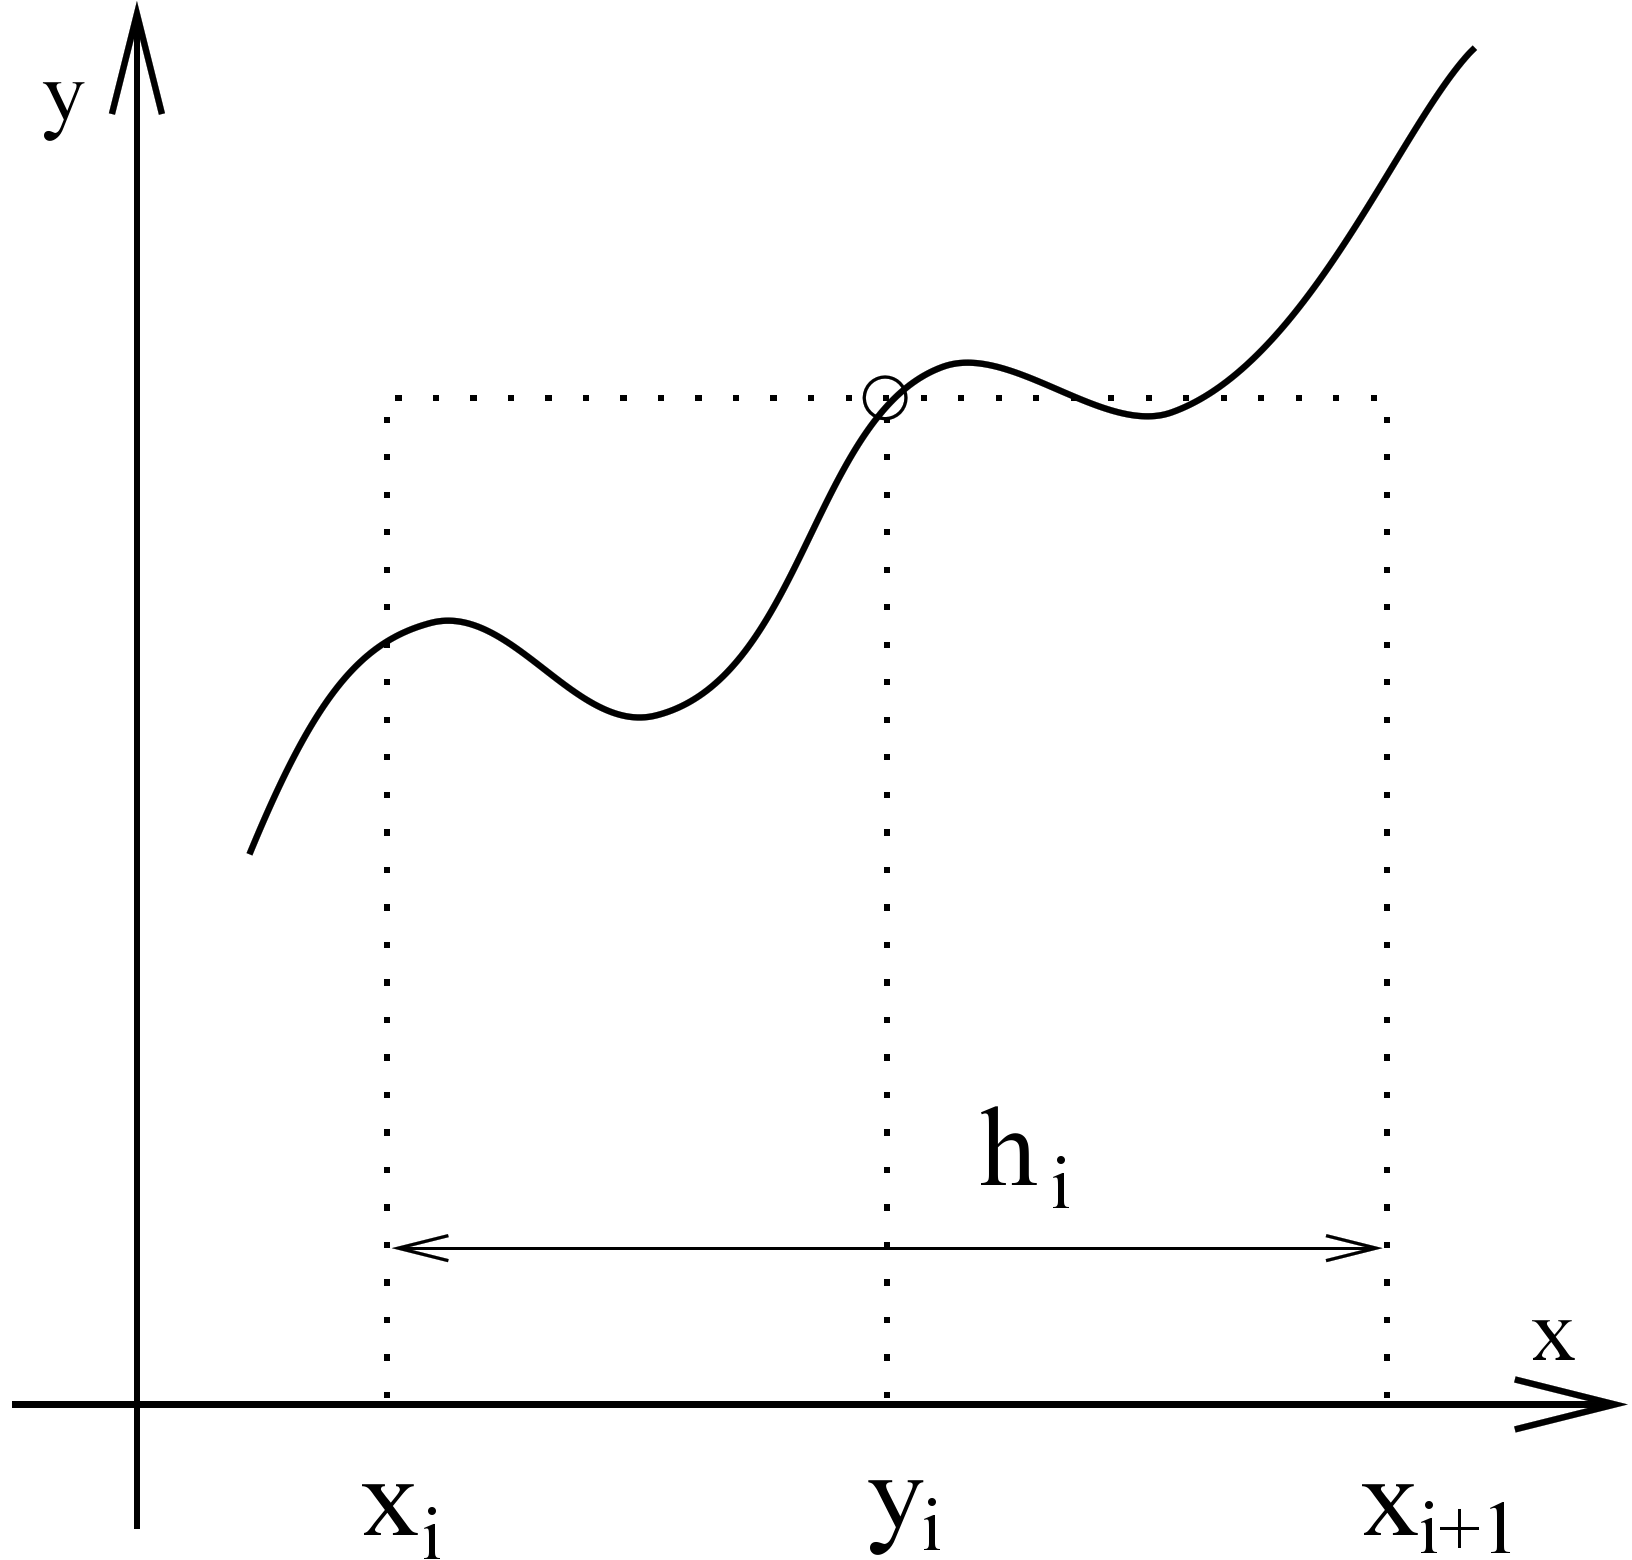
\includegraphics[width=0.4\linewidth]{img/6/image002.png}
      	\end{center}
        
		$$
y_{i}= \frac{1}{2}(x_{i}+x_{i+1}),\ \ \ f(x)=f(y_{i})+ \sum_{p=1}^{\infty}\frac{(x-y_{i})^{p}}{p!}f^{(p)}(y_{i})
		$$
        
		$$
\int_{xi}^{x_{i+1}}f(x)dx=\underbrace{y_{i}h_{i}}_{R}+\frac{1}{24}h_{i}^{3}f''(y_{i})+\frac{1}{1920}h_{i}^{5}f^{(4)}(y_{i})+\ldots
		$$
	\end{frame}
%%%%%%%%%%%%%%%%%%%%%%%%%
	\begin{frame}{Wzór trapezów}
    	$$
f(x_{i})=f(y_{i})- \frac{1}{2}h_{i}f'(y_{i})+\ldots,\ \ f(x_{i+1})=f(y_{i})+ \frac{1}{2}h_{i}f'(y_{i})+\ldots
        $$
        
		$$
\int_{a}^{b}f(x)dx=\underbrace{\frac{1}{2}[f(x_{i}) + f(x_{i+1})] \cdot h_{i}}_{T} - \frac{1}{12}h_{i}^{3} f''(y_{i})-\frac{1}{480}h_{i}^{5}f^{(4)}(y_{i})+\ldots
		$$ 
	\end{frame}
%%%%%%%%%%%%%%%%%%%%%%%%%
	\begin{frame}{Wzór Simpsona}
		$$
        \textnormal{sposób:} \left\{\begin{array}{l}
  			I = R + E + F \\
        	I = T - 2E - 4F
        \end{array}\right.
        $$
        
        $$
S = \frac{1}{6}h_{i}[f(x_{i})+4f(\frac{x_{i}+x_{i+1}}{2})+f(x_{i+1})];\ \tilde{E}=-\frac{1}{2880}h_{i}^{5}f^{(4)}(y_{i})
		$$
        oparta na interpolacji 2-go rzędu\newline ale dokładna dla funkcji sześciennych.
        
      	\begin{center}
      		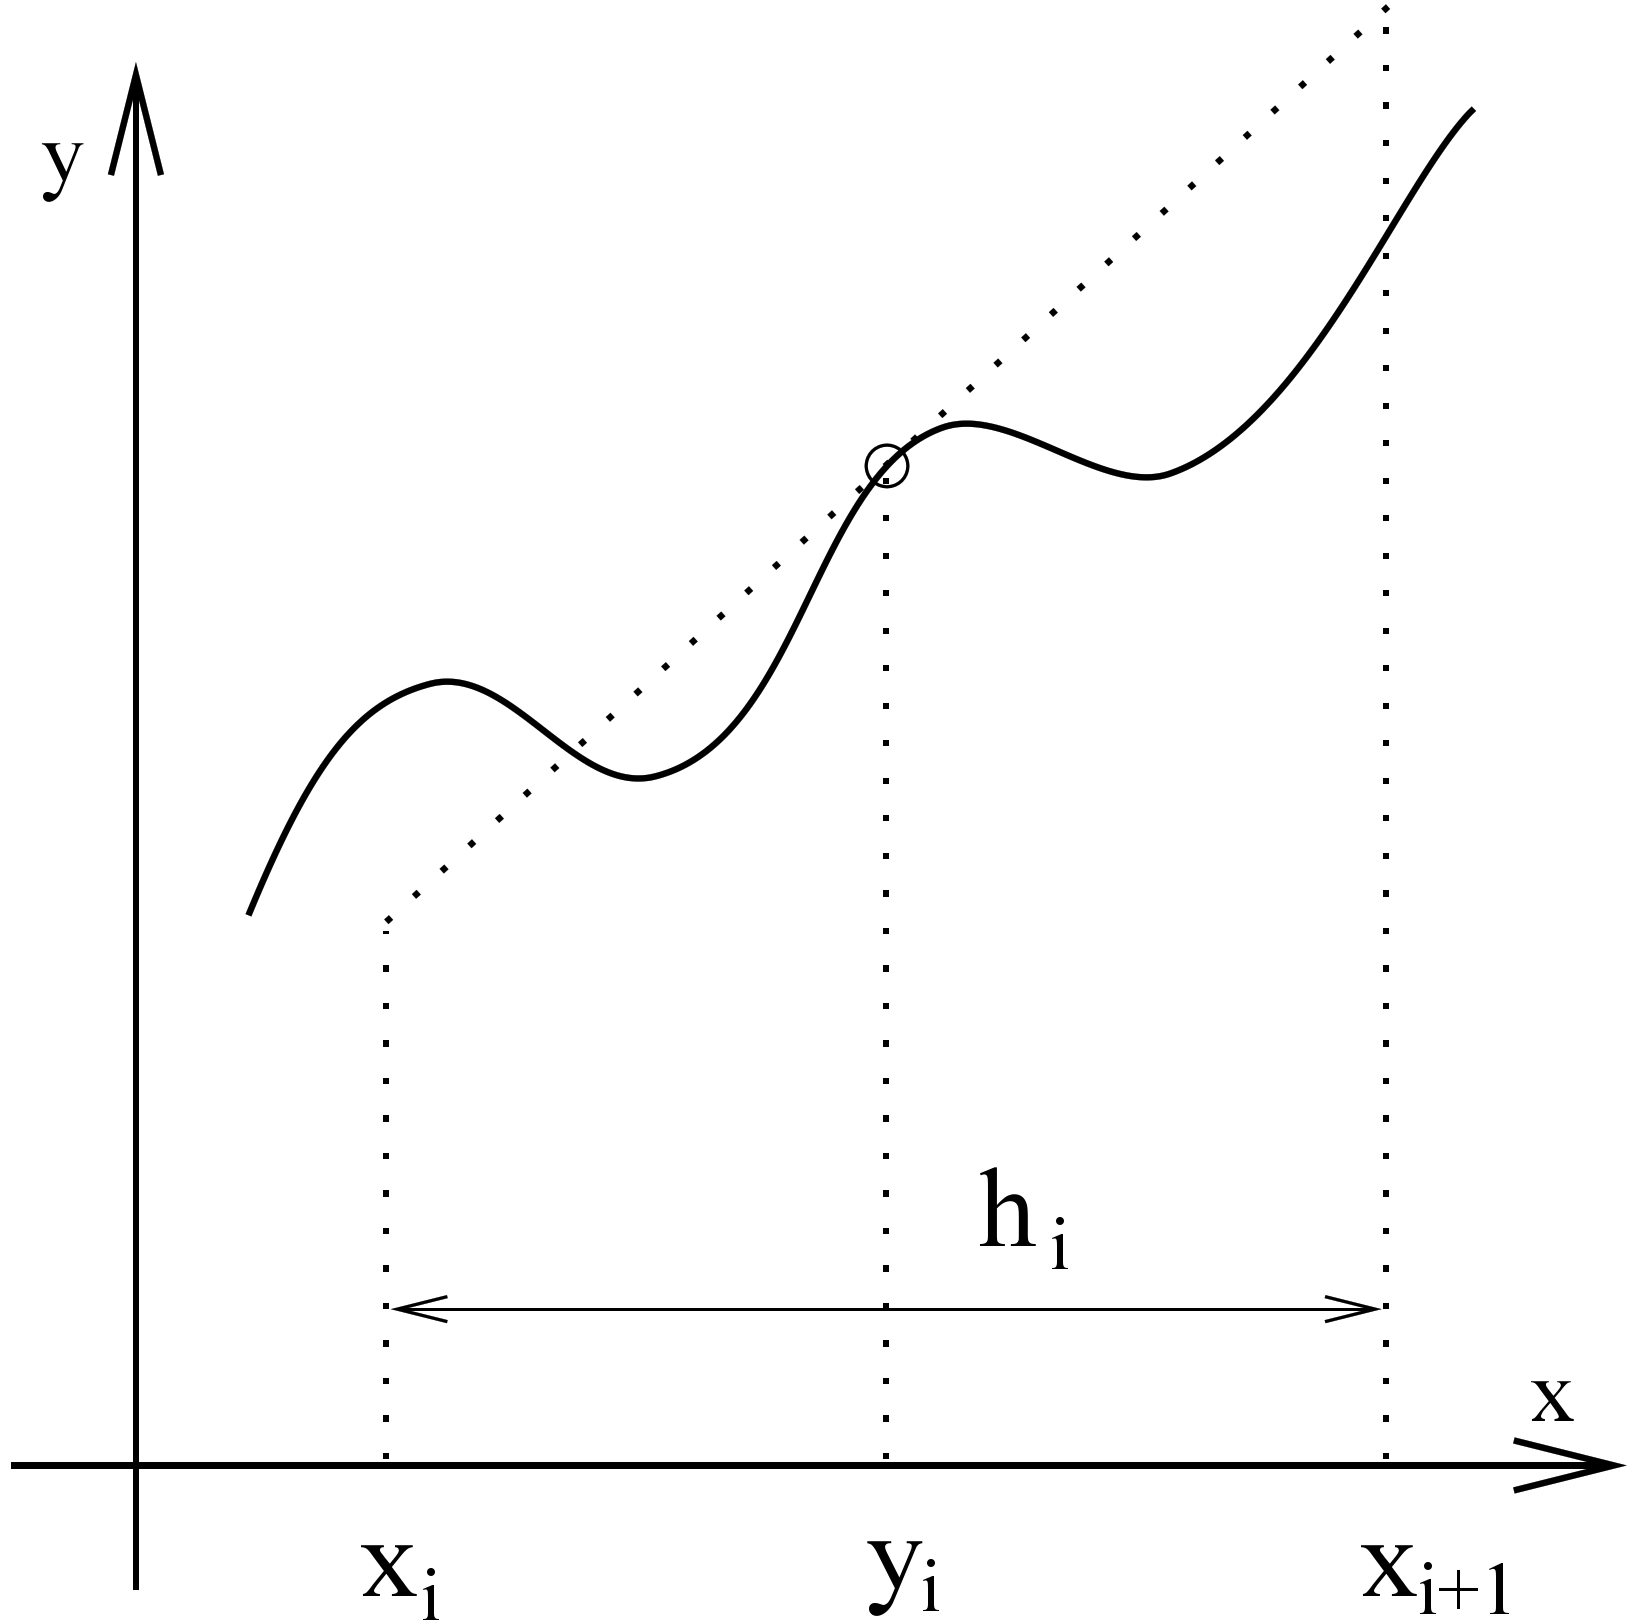
\includegraphics[width=0.35\linewidth]{img/6/image003.png}
      	\end{center}
	\end{frame}
%%%%%%%%%%%%%%%%%%%%%%%%%

	%%%%%%%%%%%%%%%%%%%%%%%
	\section{Kwadratury Newtona-Cotesa}
%%%%%%%%%%%%%%%%%%%%%%%%%
	\begin{frame}{Kwadratury Newtona-Cotesa}
		Zamiana problematycznej funkcji podcałkowej na prosty wielomian interpolujący.
		$\newline$$\newline$
		\textcolor{blue}{Charakterystyka kwadratur N-C:}
    	\begin{itemize}
    	\item wzór interpolacyjny Lagrange'a:
        \[
        f(x)=\sum_{i=0}^{n}L_{i}(x)f(x_{i})+\frac{f^{(n+1)}(\eta(x))}{(n+1)!}\prod_{j=0}^{n}(x-x_{j})
        \]
        \item węzły równoodległe
    	\end{itemize}
    	$\newline$
    	\textcolor{blue}{Uwagi:}
    	\begin{itemize}
    	\item metody prostokątów i trapezów są szczególnymi przypadkami kwadratur N-C
    	\item lepsze efekty uzyskuje się zastępując węzły równoodległe węzłami Czebyszewa
    	\end{itemize}
	\end{frame}
%%%%%%%%%%%%%%%%%%%%%%%%%
	\begin{frame}{Wzory zamknięte N-C}
    	$$
        h=\frac{b-a}{n},\ a=x_{0}<x_{1}<\ldots<x_{n}=b,\newline x_{i}=x_{0}+i\cdot h,\ i=0, 1, \ldots , n
        $$
          $$
\int_{a}^{b}f(x)dx=\sum_{i=0}^{n}a_{i}f(x_{i})+E
          $$
		
        \textbf{Liczby Cotesa:}
          $$
a_{i}=\int_{x_{0}}^{x_{n}}L_{i}(x)dx=\int_{x_{0}}^{x_{n}}\prod_{j=0,j\neq i}^{n}\frac{x-x_{j}}{x_{i}-x_{j}}dx
          $$
          \begin{itemize}
          \item wszystkie $a_{i}>0$ tylko dla $:n\leq 7, n=9$
          \item $\sum a_{i}$ =długości przedziału całkowania(dlaczego?)
          \end{itemize}
         \begin{flushright}
         	\textbf{Zadanie: pokazać}
         \end{flushright}
    
	\end{frame}
%%%%%%%%%%%%%%%%%%%%%%%%%
	\begin{frame}
    	\textbf{Błąd} \textit{E}, $\eta\in[a,\ b]$ \newline
        \begin{itemize}
        \item \textit{n-parzyste}, $f\in C^{n+2}[a,\ b]$
        $$
 		E= \frac{h^{n+3}\cdot f^{(n+2)}(\eta)}{(n+2)!}\int_{0}^{n}t^{2}(t-1)\ldots(t-n)dt
 		$$
        stopień dokładności: (n+1) 
        \item \textit{n-nieparzyste}, $f\in C^{n+1}[a,\ b]$
        $$
		E=\frac{h^{n+2}\cdot f^{(n+1)}(\eta)}{(n+1)!}\int_{0}^{n}t(t-1)\ldots(t-n)dt
 		$$
        stopień dokładności: (n)
        \end{itemize}
        \begin{flushright}
         	Zadanie, A. Ralston, Rozdz. 4 (1983)
        \end{flushright}
	\end{frame}
%%%%%%%%%%%%%%%%%%%%%%%%%
	\begin{frame}{Najczęściej używane formuły zamknięte N-C}
		a) $n=1$, Trapezoid Rule
        $$
          \int_{x_{0}}^{x_{1}}f(x)dx=\frac{h}{2}[f(x_{0})+f(x_{1})]-\frac{h^{3}}{12}f''(\eta)\ ,\ \eta\in[a,\ b]
        $$
        b) $n=2$, Simpson's Rule
      
        $$
          \int_{x_{0}}^{x_{2}}f(x)dx=\frac{h}{3}[f(x_{0})+4f(x_{1})+f(x_{2})]-\frac{h^{5}}{90}f^{(4)}(\eta)
        $$
        
	\end{frame}          
%%%%%%%%%%%%%%%%%%%%%%%%%
	\begin{frame}
        c) $n=3$, Simpson's Three-Eights Rule
        $$
          \int_{x_{0}}^{x_{3}}f(x)dx=\frac{3h}{8}[f(x_{0})+3f(x_{1})+3f(x_{2})+f(x_{3})]-\frac{3h^{5}}{80}f^{(4)}(\eta)
        $$
        d) $n=4$\newline\newline
        \scalebox{0.85}{
        $
        \displaystyle\int_{x_{0}}^{x_{4}}f(x)dx=\frac{2h}{45}[7f(x_{0})+32f(x_{1})+12f(x_{2})+32f(x_{3})+7f(x_{4})]-\frac{8h^{7}}{945}f^{(6)}(\eta))
        $
        }
	\end{frame}
%%%%%%%%%%%%%%%%%%%%%%%%%
	\begin{frame}{Wzory otwarte N-C}
		
$h=\frac{b-a}{n+2} \ \ , a=x_{-1}<x_{0}<x_{1}<\ldots<x_{n}<x_{n+1}=b,$\\ $\newline$
$x_{i}=x_{0}+i\cdot h,\ i=0, 1,\ldots,n$

   	$$
    \int_{a}^{b}f(x)dx=\int_{x_{-1}}^{x_{n+1}}f(x)dx=\sum_{i=0}^{n}a_{i}f(x_{i})+E
    $$
    
\textbf{Liczby Cotesa:} $$a_{i}=\int_{a}^{b}L_{i}(x)dx$$

wszystkie $a_{i}>0$ tylko dla $n=1$, 2, 3, 5.

	\end{frame}
%%%%%%%%%%%%%%%%%%%%%%%%%
	\begin{frame}
	
	\textbf{Błąd} $E, \eta\in[a,\ b]$
	\begin{itemize}
	\item {\it n-parzyste}, $f\in C^{n+2}[a,\ b]$
     $$
		E= \frac{h^{n+3}\cdot f^{(n+2)}(\eta)}{(n+2)!}\int_{-1}^{n+1}t^{2}(t-1)\ldots(t-n)dt,
    $$
     stopień dokładności: (n+1) 
     $\newline$
    \item {\it n-nieparzyste}, $f\in C^{n+1}[a,\ b]$
    $$
		E= \frac{h^{n+2}\cdot f^{(n+1)}(\eta)}{(n+1)!}\int_{-1}^{n+1}t(t-1)\ldots(t-n)dt,
    $$
     stopień dokładności: (n) 
	\end{itemize}
	\end{frame}
%%%%%%%%%%%%%%%%%%%%%%%%%
	\begin{frame}{Najczęściej używane kwadratury otwarte Newtona-Cotesa}
a) $n=0$ \textbf{, Midpoint Rule, Rectangle Rule}

		$$
\int_{x-1}^{x_{1}}f(x)dx=2hf(x_{0})+\frac{h^{3}}{3}f''(\eta)\ ,\ \eta\in[x_{-1},\ x_{n+1}]
		$$

b) $n=1$
		$$
\int_{x-1}^{x_{2}}f(x)dx=\frac{3h}{2}[f(x_{0})+f(x_{1})]+\frac{3h^{3}}{4}f''(\eta)
		$$

c) $n=2$ \textbf{, Milne's Rule}
		$$
\int_{x-1}^{x_{3}}f(x)dx=\frac{4h}{3}[2f(x_{0})-f(x_{1})+2f(x_{2})]+\frac{14h^{5}}{45}f^{(4)}(\eta)
		$$

d) $n=3$
		$$
\int_{x-1}^{x_{4}}f(x)dx=\frac{5h}{24} [11f(x_{0})+f(x_{1})+f(x_{2})+11f(x_{3})]+ \frac{95h^{5}}{144}f^{(4)}(\eta)
		$$
	\end{frame}
%%%%%%%%%%%%%%%%%%%%%%%%%
	\begin{frame}{Kwadratury N-C -- podsumowanie}
    \begin{itemize}
    	\item zwiększenie stopnia dokładności (otwartych i zamkniętych) przez dodanie co najmniej 2 nowych węzłów
    		
    	\item w przypadku dodania jednego punktu dla:
    	\begin{itemize}
    		\item[*] parzystej liczby węzłów $\rightarrow$ brak zmian st. dokładności,
    		\item[*] nieparzytej liczby węzłów $\rightarrow$ wzrost st. dokładności o 2
    	\end{itemize}
    	\item otwarte -- na ogół gorsze od zamkniętych, używane:
    		\begin{itemize}
    			\item[*] osobliwości w granicach przedziału
    			\item[*] w numerycznym rozwiązywaniu równań różniczkowych zwyczajnych
    		\end{itemize}
   	 	\item możliwe formuły półotwarte (półzamknięte)
    	\end{itemize}
	\end{frame}
%%%%%%%%%%%%%%%%%%%%%%%%%
	\begin{frame}
	\begin{itemize}
		\item efekty wzrostu $n$:
        \begin{itemize}
        	\item[*]  zmniejszanie stałego czynnika w $E$ , lecz wzrost rzędu pochodnej
            \item[*] trudności z oszacowaniem $E$
            \item[*] duże wartości $f^{(n+1)}(\eta)$
            \item[*] $a_{i}>0:$
            zamknięte - tylko $n=1$, 2,\ldots 7 i 9
            otwarte - tylko $n=$1, 2, 3 i 5. - złe uwarunkowanie
            \item[*] oscylacyjny charakter wielomianu interpolacyjnego (zwłaszcza, że
 			węzły są równoodległe)
            \item[*] trudne do uzyskania liczby Cotesa
        \end{itemize}
       \item $\sum_{i=1}^{n}a_{i}=(b-a)$ ($\rightarrow$ dlaczego?)
	\end{itemize}
	\end{frame}







	%%%%%%%%%%%%%%%%%%%%%%%
	\section{Złożone kwadratury Newtona-Cotesa}
	\begin{frame}{Złożone kwadratury Newtona-Cotesa}
		Wzory N-C są niedogodne dla dużych $[a,\ b]-$ {\it piecewise technique}
        \begin{center}
      		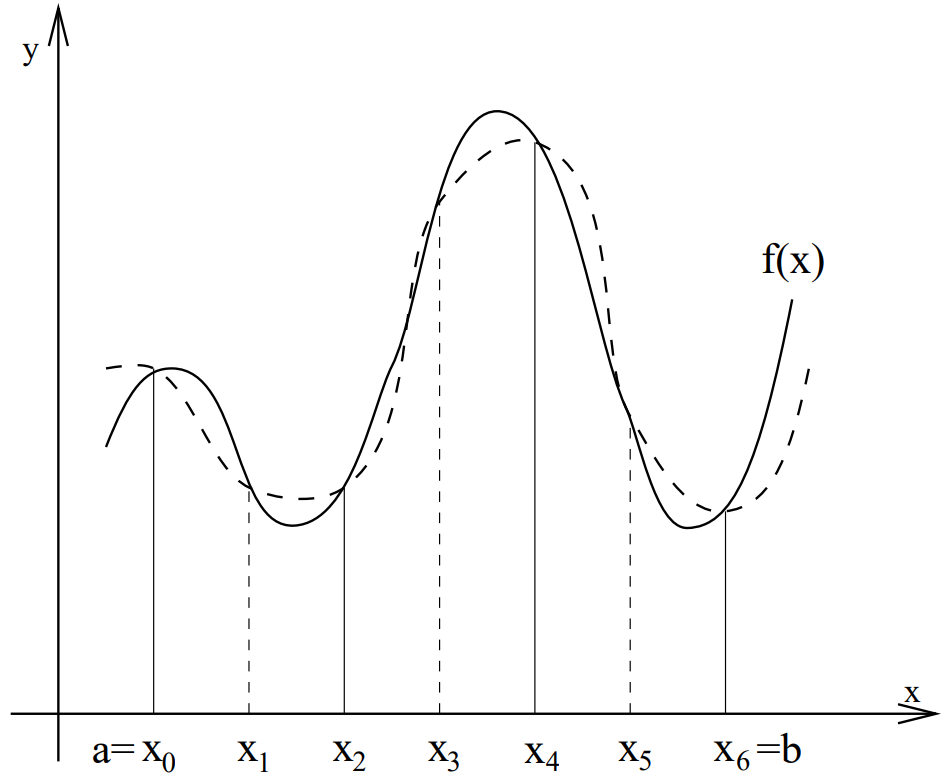
\includegraphics[width=0.6\linewidth]{img/6/image004.png}
      	\end{center}
	\end{frame}
%%%%%%%%%%%%%%%%%%%%%%%%%
	\begin{frame}
		Przedział $[a,\ b]$ podzielony na $n$ podprzedziałów $n=2m.$
        \newline
        (Simpson element. - 3 węzły)  
        $$
        h=\frac{b-a}{2m}, x_{i}=x_{0}+i\cdot h,\quad i=0, 1, 2, . . . , 2m
        $$
        \scalebox{0.85}{
          $\displaystyle
          \int_{a}^{b}f(x)dx=\sum_{j=1}^{m}\int_{x_{2j-2}}^{x_{2j}}f(x)dx=\sum_{j=1}^{m}\{\frac{h}{3}[f(x_{2j-2})+4f(x_{2j-1})+f(x_{2j})]-\frac{h^{5}}{90}f^{(4)}(\eta_{j})\}
          $
        }

        $\eta\in(x_{2j-2},\ x_{2j})$
        \newline
        \newline
        $f(x_{2j})$ występuje w składowych dla: $[x_{2j-2},\ x_{2j}]  [x_{2j},\ x_{2j+2}]$ i stąd:
        \newline

        \scalebox{0.9}{
          $\displaystyle
          \int_{a}^{b}f(x)dx=\frac{h}{3}[f(x_{0})+4\sum_{j=1}^{m}f(x_{2j-1})+\sum_{j=1}^{m-1}f(x_{2j})+f(x_{2m})]-\frac{h^{5}}{90}\sum_{j=1}^{m}f^{(4)}(\eta_{j})
          $
        }
	\end{frame}
%%%%%%%%%%%%%%%%%%%%%%%%%
	\begin{frame}{Błąd dla wzoru złożonego}
      \textbf{z tw. o wartości średniej: ( $f^{(4)}$ - ciągła )}
      $$
      \min_{x\in[a,b]}f^{(4)}(x)\leq f^{(4)}(\eta_{j})\leq \max_{x\in[a,b]}f^{(4)}(x) ,\quad \eta_{j}\in(x_{2j-2},\ x_{2j})
      $$
      \newline
	  dla każdego przedziału w wyniku dodawania:
      \begin{center}
        $\displaystyle
        m\cdot\min_{x\in[a,b]}f^{(4)}(x)\leq\sum_{j=1}^{m}f^{(4)}(\eta_{j})\leq m\cdot \max_{x\in[a,b]}f^{(4)}(x),
        $
        \newline
        $\displaystyle
        \min_{x\in[a,b]}f^{(4)}(x)\leq\frac{1}{m}\sum_{j=1}^{m}f^{(4)}(\eta_{j})\leq \max_{x\in[a,b]}f^{(4)}(x),
        $
      \end{center}
        
    \end{frame}
%%%%%%%%%%%%%%%%%%%%%%%%%
	\begin{frame}
      $$
      \textnormal{(z tw.) }\exists\mu\in(a,\ b) :\quad f^{(4)}(\mu)=\frac{1}{m}\sum_{j=1}^{m}f^{(4)}(n_{j}) \quad \Rightarrow
      $$

      $\displaystyle
      \qquad\quad E=-\frac{h^{5}}{90} \cdot m\cdot f^{(4)}(\mu) ,\quad m= \frac{b-a}{2h} \quad \Rightarrow
      $
      \begin{exampleblock}{}
      	\[
        	E=-\frac{h^{4}(b-a)}{180}f^{(4)}(\mu)
        \]
      \end{exampleblock}
%       \begin{center}
%       \fbox{$E=-\displaystyle $}
%       \end{center}
    \end{frame}
%%%%%%%%%%%%%%%%%%%%%%%%%
	\begin{frame}{Wpływ błędu wyznaczania $f(x)$}
        $$
        f(x_{i})=f^{\star}(x_{i})+e_{i};\quad i=0, 1, 2, . . ., 2m
        $$
        \newline
        (błąd zaokrąglenia $|\epsilon_{i}|<\epsilon$)
        \newline
		błąd wzoru złożonego:
        \scalebox{0.72}{
          $\displaystyle \Upsilon=|\frac{h}{3}[e_{0}+4\sum_{j=1}^{m}e_{2j-1}+2\sum_{j=1}^{m-1}e_{2j}+e_{2m}]|\leq\frac{h}{3}[\epsilon+4m\epsilon+2(m+1)\epsilon+\epsilon]=2mh\epsilon= \fbox{$(b-a)\cdot\epsilon$}$
		}
        
        \quad $\bullet$ nie zalezy od $h$
        
		\quad $\bullet$ $h\rightarrow 0$ to stabilna
        
		\quad $\bullet$ nie mylić z błędem metody!!!!
        
		\quad $\bullet$ stabilność metody ze względu na błędy zaokrągleń (reprezentacji) - cecha procedur calkowania numerycznego!\newline (nie ma jej np. różniczkowanie!)\newline

		\textbf{{\it Zadanie}: wzory złożone dla trapezów i prostokątów}
        
    \end{frame}
%%%%%%%%%%%%%%%%%%%%%%%%%
	%%%%%%%%%%%%%%%%%%%%%%%
	\section{Całkowanie adaptacyjne}
	\begin{frame}{Całkowanie adaptacyjne}
		
      wzory złożone - Węzly równoodległe,
      funkcje mogą mieć w przedziale całkowania różny (przedziałami) przebieg:
      $\newline$
      \begin{itemize}
      \item wolnozmienne
      \item oscylacyjne
      \end{itemize}
      $\newline$
      potrzebna jest \textit{procedura rozpoznająca obszary: dobierająca krok!}
      \end{frame}
%%%%%%%%%%%%%%%%%%%%%%%%%
      \begin{frame}
      
        Liczymy całkę $\displaystyle \int_{a}^{b}f(x)d_{x},$\quad z dokładnością $\epsilon>0$

        1. $m=1$, krok $h=\displaystyle \frac{b-a}{2}$

      
        $$ 
        \int_{a}^{b}f(x)dx=\underbrace{\frac{h}{3}[f(a)+4f(a+h)+f(b)]}_{S(a,b)} - \underbrace{\frac{h^{5}}{90}f^{(4)}(\mu)}_{\alpha} ;\quad \mu\in(a,\ b)
        $$
      \end{frame}
%%%%%%%%%%%%%%%%%%%%%%%%%
      \begin{frame}
      
		2. $m=2$, krok $\displaystyle \frac{h}{2}=\frac{b-a}{4}$ $\newline$
        \scalebox{0.85}{
            $
                \displaystyle \int_{a}^{b}f(x)dx=\frac{h}{6}\underbrace{[f(a)+4f(a+\frac{h}{2})+f(a+h)}_{S(a,\frac{a+b}{2})}+\underbrace{(a+h)+4f(a+\frac{3}{4}h)+f(b)]}_{S(\frac{a+b}{2},b)} - 
            $
        }
        \begin{center}
          \scalebox{0.85}{
            $
            \displaystyle(\frac{h}{2})^{4}\frac{b-a}{180}f^{(4)}(\mu^{\star}) , \mu^{\star}\in(a,\ b)
            $
          }
        \end{center}
        przyjmijmy, że: $f^{(4)}(\mu)\approx f^{(4)}(\mu^{\star})$

        \textbf{Z porównania 1. i 2. :}
        $$
        S(a,b)-\alpha\approx S(a,\ \frac{a+b}{2})+S(\frac{a+b}{2},\ b)-\frac{1}{16}\alpha \quad\Rightarrow
        $$

        $$
        \alpha=\frac{16}{15}[S(a,\ b)-S(a,\ \frac{a+b}{2})-S(\frac{a+b}{2},\ b)]
        $$

	\end{frame}
%%%%%%%%%%%%%%%%%%%%%%%%%
	\begin{frame}
    	uzyskujemy:
        $\newline$
      \scalebox{0.8}{
          $|\displaystyle \int_{a}^{b}f(x)dx-S(a,\ \frac{a+b}{2})-S(\frac{a+b}{2},\ b)|\approx\frac{1}{15}|s(a,\ b)-S(a,\ \frac{a+b}{2})-S(\frac{a+b}{2},\ b)|$ 
      }
      $\newline$
      \scalebox{0.9}{
      	(lewa strona równania powinna być równa $\epsilon$)
      }
	  $\newline$
      
      Wtedy:
      $$
	      |S(a,\ b)-S(a,\ \frac{a+b}{2})-S(\frac{a+b}{2},\ b)|<15\epsilon \quad(*)
      $$
	\end{frame}
%%%%%%%%%%%%%%%%%%%%%%%%%
	\begin{frame}
    	Mamy więc sposób postępowania:
        $\newline$
        \begin{itemize}
          \item gdy spelnione $(*)$ $\displaystyle \Rightarrow S(a,\ \frac{a+b}{2})+S(\frac{a+b}{2},\ b)\newline$ 
          przybliża całke $\displaystyle\int_{a}^{b}f(x)dx$ z dokladnością $\epsilon$, STOP
			
          \item nie jest spełnione $(*)$ stosujemy procedurę oceny błędu do przedziaów
$[a,\displaystyle \ \frac{a+b}{2}], [\displaystyle \frac{a+b}{2},\ b]$ w każdym z nich: 	$\displaystyle \epsilon'=\frac{\epsilon}{2}$
          
          \item połowienie podprzedziałów i wyznaczanie $S$
          
          \item ten, na którym odpowiednik $(*)$ nie jest spełniony znów połowimy
            
        \end{itemize}
	\end{frame}
%%%%%%%%%%%%%%%%%%%%%%%%%























	%%%%%%%%%%%%%%%%%%%%%%%
	\section{Schemat całkowania Romberga}
	\begin{frame}{Schemat całkowania Romberga}
    	
      Całkowity błąd złożonej kwadratury trapezów:
      $\newline$
      $$E=\displaystyle \sum_{i=1}^{\infty}a_{i}h^{2i}$$
	  $$a_{i}=a_{i}(a,\ b,\ f(x)) , \ \ \textbf{nie zależy od h!}$$
    \end{frame}
%%%%%%%%%%%%%%%%%%%%%%%%%
	\begin{frame}
    		
  	  	$\hfill${\it Zadanie}: p. Ralston
	
      	Aby tak było $\rightarrow$ $f\in C^{\infty}[a,\ b]; \quad I =\displaystyle \int_{a}^{b}f(x)dx$;

      	$T_{a,j}$ -\ wynik kwadratury trapezów dla $h_{j}=\displaystyle  \frac{b-a}{2j}$
		$\newline$
        
	  	\textbf{1-szy krok:}

		$\left\{\begin{array}{l}
			I-T_{0,j}=a_{2}h_{j}^{2}+a_{4}h_{j}^{4}+\ldots\\
			I-T_{0,j+1}=a_{2}h_{j+1}^{2}+a_{4}h_{j+1}^{4}+\ldots\quad\ |\rightarrow h_{j+1}=\frac{h_{j}}{2};*4,\ -,\ /3
		\end{array}\right.$ 
		$\newline$
        ekstrapolacja Richardsona daje:
        $$
        	I-\displaystyle \underbrace{\frac{1}{3}[4T_{0,j+1}-T_{0,j}]}_{T_{1,j}}=b_{4}h_{j}^{4}+b_{6}h_{j}^{6}+\ldots
        $$
        $T_{1,j} \equiv$ wzór Simpsona dla $2^{j}$ podprzedziałów.

        $\hfill${\it Zadanie}: Pokazać

    \end{frame}
%%%%%%%%%%%%%%%%%%%%%%%%%
	\begin{frame}
    	\textbf{2-gi krok:}
        
        $\left\{\begin{array}{l}
        	I-T_{1,j}=b_{4}h_{j}^{2}+b_{6}h_{j}^{4}+\ldots \\
        	I-T_{1,j+1}=b_{4}h_{j+1}^{2}+b_{6}h_{j+1}^{4}+\ldots\quad\;*4;-;/3
        \end{array}\right.$
        
        $$
        I-\displaystyle \underbrace{\frac{1}{15}[16T_{1,j+1}-T_{1,j}]}_{T_{2,j}}=c_{6}h_{j}^{6}+c_{8}h_{j}^{8}+\ldots
        $$
        
        I ogólnie:
        mając
        \begin{center}
        $T_{0,j},\quad j=0$, 1, . . . , $m$
        \end{center}
        tworzymy:
        
        $$
        	T_{i,j}=\displaystyle \frac{1}{4^{i}-1}(4^{i}T_{i-1,j-1}-T_{i-1,j}) ,\quad i, j=0, 1, 2, . . .   
        $$
        $\hfill${\it Zadanie}: Udowodnić
    
    \end{frame}
%%%%%%%%%%%%%%%%%%%%%%%%%
	\begin{frame}{Romberg $T$-table:}
    	\scalebox{0.92}{
		$\begin{array}{ccccccccccc}
          	T_{0,0} \\
        	\downarrow & \searrow \\
        	T_{0,1} & \rightarrow & T_{1,0} \\
            \downarrow & \searrow & \downarrow & \searrow \\
            T_{0,2} & \rightarrow & T_{1,1} & \rightarrow & T_{2,0} \\
            \downarrow & \searrow & \downarrow & \searrow & \downarrow & \searrow \\
            T_{0,3} & \rightarrow & T_{1,2} & \rightarrow & T_{2,1} & \rightarrow & T_{3,0} \\
            & \ldots \\
            \downarrow & \searrow & \downarrow & \searrow & \downarrow & \searrow & & \searrow \\
            T_{0,m-1} & \rightarrow & T_{1,m-2} & \rightarrow & T_{2,m-3} & \rightarrow & T_{3,m-4} & \ldots & T_{m-1,0} \\
            \downarrow & \searrow & \downarrow & \searrow & \downarrow & \searrow & & \searrow & \downarrow & \searrow \\
            T_{0,m} & \rightarrow & T_{1,m-1} & \rightarrow & T_{2,m-2} & \rightarrow & T_{3,m-3} & \ldots & T_{m-1,1} & \rightarrow &  T_{m,0}\\
            
        \end{array}$
        }
        $\newline$
        Sposób wypełniania wierszy tablicy $T$: (wystarczy 1 wiersz)
    \end{frame}
%%%%%%%%%%%%%%%%%%%%%%%%%
	\begin{frame}
    	\textbf{- 1-sza iteracja:}
        $\newline$
    	$\begin{array}{ccc}
        	T_{0,0} \\
            T_{0,0} & \rightarrow & T_{0,1} \\
            \downarrow & \swarrow \\
            T_{1,0} & & T_{0,1}
        \end{array}$
        
        $\newline$
        
    	\textbf{- 2-ga iteracja:}
        
        $\begin{array}{cccccc}
            T_{0,0} & \rightarrow & T_{0,1} & \rightarrow & T_{0,2} \\
            \downarrow & \swarrow &\downarrow \\
            T_{1,0} & & T_{1,1} & & T_{0,2} \\
            \downarrow & \swarrow \\
            T_{2,0} & & T_{1,1} & & T_{0,2} \\
        \end{array}$
    \end{frame}
%%%%%%%%%%%%%%%%%%%%%%%%%
	\begin{frame}
    	\textcolor{blue}{Zbieżność całkowania Romberga} $\rightarrow$ patrz Ralston $\newline$

        \textbf{Ogólnie:}$\newline$ Im wyższe $\mathrm{i}, h^{i}\rightarrow$ tym większe $f^{i}(\eta)$ $\newline$
		ale -- w całkowaniu trapezów $\rightarrow$ zbieżność! $\newline$
        
		\textbf{Gdy $f(x)\in C^{\infty}[a,\ b]$,  to}:
		\begin{itemize}
		\item w kolumnach $\displaystyle \lim_{l\rightarrow\infty}T_{p,l}\rightarrow I$;\quad $w\ (p+1)$ szybciej niż w $p$

		\item ciąg diagonalny $T_{i,i}$ szybciej zbieżny do I niż ciągi w kolumnach
		\end{itemize}
       
		Stąd warunek zakończenia:
        \begin{center}
        	$|T_{m,0}-T_{m-1,0}|<\delta \cdot |T_{m,0}|, \delta-$ {\it zadane}.
        \end{center}
        
        Reszta schematu Romberga:
        \begin{center}
        	$E=c(i,\ j)\cdot h^{2j+2}\cdot f^{2j+2}(\eta)$
        
		$c(i,\ j)$ - stała malejąca z $i$, $j$\quad $h=\displaystyle \frac{b-a}{2^{i+j}}.$
		\end{center}

    \end{frame}
%%%%%%%%%%%%%%%%%%%%%%%%%
    \begin{frame}
    \textbf{Uwagi:}
    \begin{itemize}
    	\item Schemat Romberga wymaga, by błąd kwadratury w  $i$-tym wierszu:
        \begin{center}
        	$E=\displaystyle \sum_{l=1}^{i}a_{l}h_{i}^{2l}+O(h_{i}^{2i+2})\ ,\quad\ f\in C^{2i+2}[a,\ b]$   
        \end{center}
W procedurze powinno to być sprawdzane!

\item Procedury całkowania Romberga mogą być adaptacyjne.
\end{itemize}
    \end{frame}
%%%%%%%%%%%%%%%%%%%%%%%%%
		
	%%%%%%%%%%%%%%%%%%%%%%%
	\section{Kwadratury Gaussa}
\newcommand\myeq{\stackrel{\mathclap{\normalfont\mbox{def}}}{=}}
  \begin{frame}{Wielomiany ortogonalne - uzupełnienie}
      Funkcja wagowa: $w(x)$ na $[a,b]$
      \begin{itemize}
          \item całkowalna na $[a,b]$
          \item $w(x) \geq 0 \ $ $\forall x \in [a,b] \ $,
              $w \neq 0 \ $ $\forall$ podprzedziału $[a,b]$
      \end{itemize}
      \begin{exampleblock}{Definicja}
          \textit{Iloczyn skalarny:}
          \[
              <f | g> \ \myeq  \ \int_{a}^{b} w(x) \cdot f(x) \cdot g(x) dx
          \]
      \end{exampleblock}
  \end{frame}
  %%%%%%%%%%%%%%%%%%%%%%%%%%%%%%%%
  \begin{frame}
      \begin{exampleblock}{Definicja}
          \textit{wielomiany ortogonalne i znormalizowane} 
          - f, g orogonalne gdy
          $\newline$
          $<f|g>=0$
          f, g - znormalizowane gdy $<f|f>=1$
      \end{exampleblock}
      \begin{exampleblock}{Definicja}
          \textit{zbiór ortonormalny} - zbiór funkcji wzajemnie 
          ortogonalnych i indywidualnie znormalizowanych
      \end{exampleblock}
      \begin{exampleblock}{Definicja}
       \textit{zbiór liniowo zależny i liniowo niezależny} - 
       $\newline$
       $\{\varphi_{i}\}_{i=0}^{n}- {\it ortogonalny}: 
          \ \ 
       <\varphi_{j}|\varphi_{k}>=\alpha_{j}\cdot\delta_{jk}$
       $\newline$
       Zbiór funkcji $\{ \varphi_{i}\}_{i=0}^{n}$ jest liniowo niezależny
       na $[a,b]$:
       \[
       (\forall x\in[a,\ b]\ :\ \sum_{i=0}^{n}c_{i}\varphi_{i}(x)=0) 
       \Rightarrow c_{0}=c_{1}=\ldots=c_{n}=0
       \]
       w przeciwnym przypadku - zbiór ten jest liniowo zależny
      \end{exampleblock}
  \end{frame}
  %%%%%%%%%%%%%%%%%%%%%%%%%%%%%%%%%%%
  \begin{frame}
      \begin{block}{Twierdzenie liniowa niezależność zbioru wielominaów
      stopnia $\leq n$}
          \begin{large}
              \textbf{Założenia:}
          \end{large}
          $\newline$
          $\varphi_{i}$ - wielomian stopnia j, $j=0,1,\ldots , n$
          $\newline$
          \begin{large}
              \textbf{Teza:}
          \end{large}
          $\newline$
          $\{\varphi_{i}\}_{i=0}^{n}$ - jest liniowo niezależny na 
          $\forall [a,b], \ \ b > a$
      \end{block}
      $\newline$
      \begin{block}{Zadanie}
          Dowód twierdzenia
      \end{block}
  \end{frame}
  %%%%%%%%%%%%%%%%%%%%%%%%%%%%%%%%%%%%
  \begin{frame}
      \begin{large}
          \textbf{Wniosek:}
      \end{large}
      $\newline$
      Dowolny wielomian stopnia $k \leq n$:
      \[
          Q_{k}(x)= \sum_{j=0}^{k}c_{j}\varphi_{k}(x)\ 
          \ \ (\exists\{c_{j}\})
      \]
      konstruowanie zbioru wielomianów ortogonalnych 
      $\{\varphi_{i}\}_{i=0}^{n}$:
      \[
          [a,b], \ \ w(x)
      \]

      \begin{block}{Zadanie}
          Pokazać, że są rzeczywiście ortogonalne
      \end{block}
      \[
       \varphi_{0}(x)=1; \ \ (\varphi_{-1}(x)=0)
      \]
      \[
       \varphi_{i+1}(x)=(x-
       \frac{<x\cdot\varphi_{i}|\varphi_{i}>}
       {<\varphi_{i} | \varphi_{i}>})\cdot\varphi_{i}(x)-
       \frac{<\varphi_{i} | \varphi_{i}>}{<\varphi_{i-1} | \varphi_{i-
       1}>}\varphi_{i-1}(x)
      \]
  \end{frame}
  %%%%%%%%%%%%%%%%%%%%%%%%%%%
  \begin{frame}
      \begin{block}{Twierdzenie o zerach wielominaów ortogonalnych}
          \begin{large}
              \textbf{Założenia:}
          \end{large}
          $\newline$
          $\{\varphi_{i}\}_{i=0}^{n}$ - zbiór wielomianów ortogonalnych na
          $[a,b]$, (względem $w(x))$
          $\newline$
          $\varphi_{k}(x) , k=0, 1, . . ., n$
          $\newline$
          \begin{large}
              \textbf{Teza:}
          \end{large}
          $\newline$
          $\varphi_{k}(x) , \ k\geq 1$ ma $k$ różnych zer i leżą one w 
          $(a,b)$
          $\newline$
          zera $\varphi_{j-1}(x)$ i $\varphi_{j}(x)$ występują na przemian
      \end{block}
  \end{frame}
  %%%%%%%%%%%%%%%%%%%%%%%%%%%%%%%%%%%%%%%%
  \begin{frame}{Ograniczenia kwadratur Newtona-Cotesa}
      \begin{itemize}
      \item węzły $x_{0},x_{1},\ldots , x_{n}$ równoległe, $h, \ f$ - 
      stablicowane
      \item $\int_{a}^{b}f(x)dx\approx\sum_{i=0}^{n}a_{i}f(x_{i})$
      $\newline$
      $x_{i}$ - zadane
      $\newline$
      $a_{i}$ - dobór wielomianu stopnia $\leq n $
      \end{itemize}
  \end{frame}
  %%%%%%%%%%%%%%%%%%%%%%%%%%%%%%%%%%%%%%%%%
  \begin{frame}{Podstawowe cechy kwadratur Gaussa}
      \begin{itemize}
      \item możliwość doboru $a_{i}$ i $x_{i}$, $i=1,2,\ldots,n$
          więc można uzyskać stopień dokładności $2n-1$
      \item szersza klasa funkcji podcałkowych (w sposób naturlany):
      \end{itemize}
      \[
          \int_{a}^{b}w(x)f(x)dx\approx\sum_{i=0}a_{i}f(x_{i})n
      \]
      waga - np. do usunięcia całkowalnej osobliwości
  \end{frame}
  %%%%%%%%%%%%%%%%%%%%%%%%%%%%%%%%%%%%%%%%%%
  \begin{frame}
      \begin{block}{Podstawowe twierdzenie kwadratur Gaussa}
          Odcięte ${x_{i}}$ n-punktowej kwadratury Gaussa z funkcją ważącą 
          $w(x)$ w $[a,b]$ są zerami wielomianu ortogonalnego
          $\varphi_{n}(x)$ dla tego samego przedziału i tej samej funkcji
          ważącej
          $\newline$
          $\newline$
          $\{\varphi_{i}\}_{i=0}^{n}$ - zbiór wielomianów ortogonalnych w 
          $[a,b]$
          $\newline$
          $\varphi_{n}(x)$ - ma $n$ różnych zer $x_{1},x_{2}, \ldots, 
          \ \ n \in (a,b)$
          \[
              f(x)= \sum_{i=1}^{n}\prod_{j=1,j\neq 
              i}^{n}\frac{x-x_{j}}{x_{i}-x_{j}}f(x_{i})+\frac{f^{(n)}
              (\eta(x))}
              {n!}\prod_{i=1}^{n}(x-x_{i})
          \]
          \[
           (*) \int_{a}^{b} w(x)f(x)dx \approx \sum_{i=1}^{n}a_{i}f(x_{i}),
           \ \ \ a_{i}=\int_{a}^{b} w(x)L_{i}(x)dx
          \]
          stopeiń dokładności $\leq n-1$ bo $f^{n}(\eta)$
      \end{block}
  \end{frame}
  %%%%%%%%%%%%%%%%%%%%%%%%%%%%%%%
  \begin{frame}{Twierdzenie o stopniu dokładności kwadratur Gaussa}
      \begin{block}{Twierdzenie stopień dokładności kwadratury Gaussa}
      \begin{large}
              \textbf{Teza:}
          \end{large}
      $\newline$
      {\it Kwadratura ma stopień dokładności $2n-1$};
      {\it tzn. jest doktadna dla wielomianu}:

      $P(x)=Q(x)\cdot\varphi_{n}(x)+R(x)$ ;\quad $Q, R-${\it stopnia} $<n. $

      \end{block}
  \end{frame}
  %%%%%%%%%%%%%%%%%%%%%%%%%%%%%%%
  \begin{frame}
	\begin{block}{Twierdzenie stopień dokładności kwadratury Gaussa}
      \begin{large}
              \textbf{Dowód:}
          \end{large}
      $\newline$
          $$(**) Q(x)=\displaystyle \sum_{i=1}^{n-1}d_{i}\varphi_{i}(x)$$
          $$
          \int_{a}^{b}w(x)P(x)dx=\underbrace{\int_{a}^{b}w(x)\overbrace{Q(x)}^{wstaw.(**)}\varphi_{n}(x)dx}_{(***)}+\int_{a}^{b}w(x)R(x)dx
          $$
          $$
          (***)=\sum_{i=1}^{n-1}d_{i}\int_{a}^{b}w(x)\varphi_{i}\varphi_{n}(x)dx=\alpha\cdot\delta_{i,n}=0\quad (i<n)
          $$

      \end{block}

  \end{frame}
  %%%%%%%%%%%%%%%%%%%%%%%%%%%%%%%
   \begin{frame}
		\begin{block}{Twierdzenie stopień dokładności kwadratury Gaussa}
     		
          \textbf{czyli:}
          $$
          \int_{a}^{b}w(x)\underbrace{P(x)}_{2n-1}dx=\int_{a}^{b}w(x)\underbrace{R(x)}_{< n} dx=\sum_{i=1}^{n}a_{i}R_{i}+0
          $$
          $\quad\rightarrow R_{i}$ stopnia $<n$, kwadratura ma przynajmniej taki
          stopień \quad dokladności.

          Z drugiej strony: $x_{i}, i=1$, 2, . . . , $n$ -- pierwiastki $\varphi_{n}(x)$
          tzn.
          $$
          P(x_{i})=Q(x_{i})\cdot\varphi_{n}(x_{i})+R(x_{i})=0+R(x_{i})=R(x_{i})
          $$
          co oznacza, że kwadratura jest dokładna dla $P_{2n-1}(x)$ :
          $$\int_{a}^{b}w(x)P_{2n-1}(x)dx=\sum_{i=1}^{n}a_{i}P(x_{i})$$
     	\end{block}
  \end{frame}
  %%%%%%%%%%%%%%%%%%%%%%%%%%%%%%%
  \begin{frame}{Wagi $a_{1}, a_{2}, \ldots, a_{n}$}
     znając odcięte $x_{1}, x_{2}$, . . . , $x_{n}\Rightarrow$ z układu równań:
     
  	\[
    \begin{bmatrix}
    	\varphi_{0}(x_{1}) && \ldots &&  \varphi_{0}(x_{n}) \\
            \vdots  \\
            \varphi_{n-2}(x_{1})  && \ldots && \varphi_{n-2}(x_{n})\\
            \varphi_{n-1}(x_{1}) && \ldots && \varphi_{n-1}(x_{n})
    \end{bmatrix}
    \cdot
    \begin{bmatrix}
        	a_{1} \\
            a_{2} \\
            \vdots \\
            a_{n}
    \end{bmatrix}
    =
    \begin{bmatrix}
        	\int_{a}^{b} w(x)\varphi_{0}(x)dx \\
            0 \\
            \vdots \\
            0
    \end{bmatrix}
    \]
    zera w wektorze z prawej strony powyższego równania - bo $\newline$ $\varphi_{1}(x)$ , . . . , $\varphi_{n-1}(x)$ są ortogonalne do $\varphi_{0}(x)$ -- stałej!
    $\newline$
    W układzie -- tylko dokładne dla wielomianów ortogonalnych stopnia $n-1!!$
    \begin{block}{Zadanie}
    	Wyprowadzić 2 i 3-punktowe wzory Gaussa - wprost.
    \end{block}

  \end{frame}
  %%%%%%%%%%%%%%%%%%%%%%%%%%%
  \begin{frame}
  	\begin{figure}[h]
			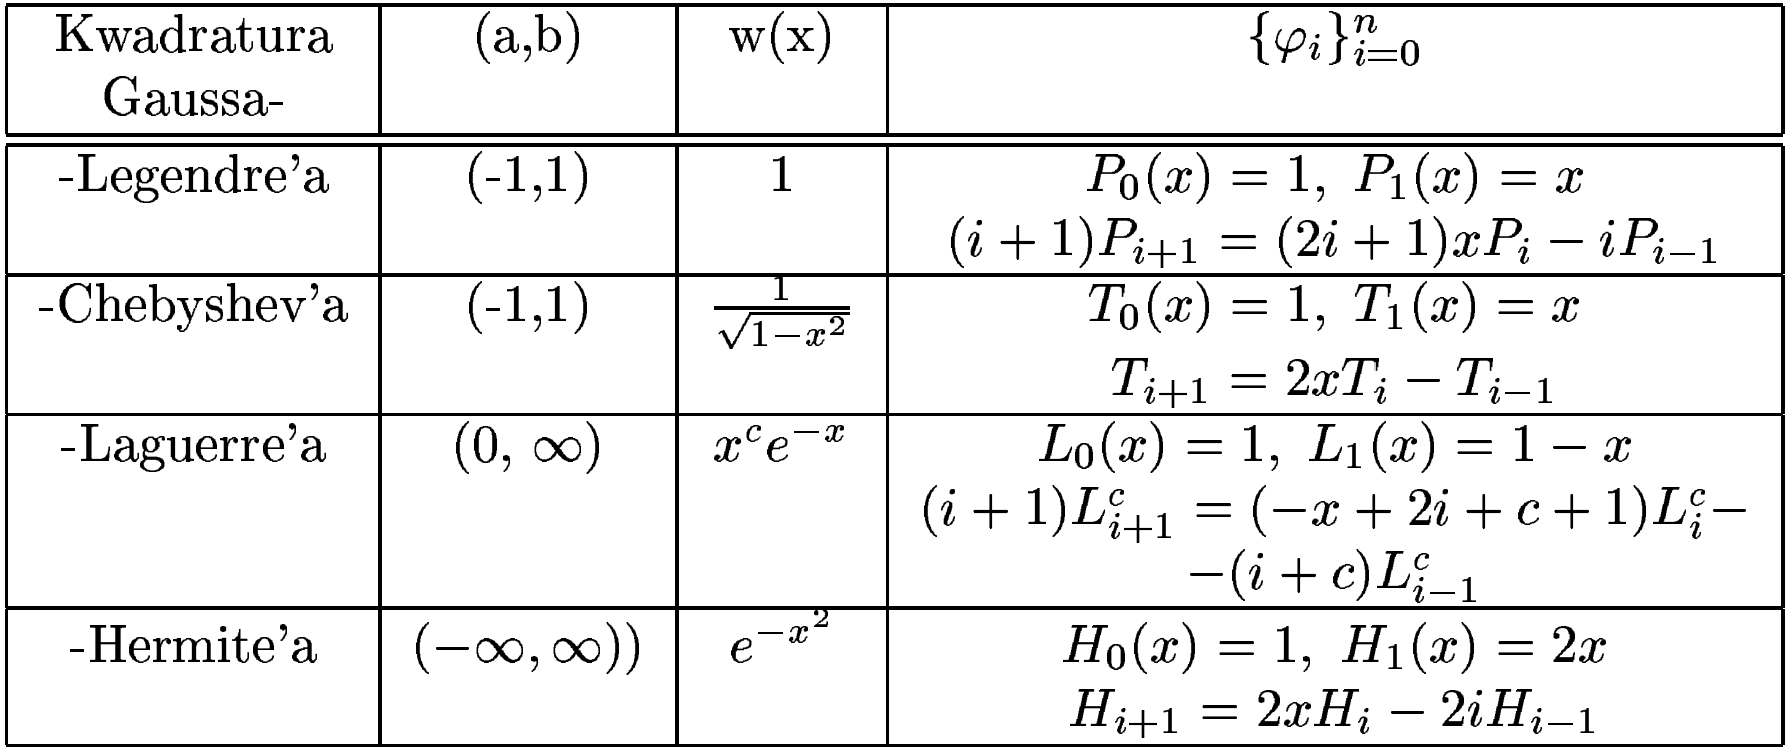
\includegraphics[width=.95\linewidth]{img/6/6_03}
		\end{figure}
  \end{frame}



























	%%%%%%%%%%%%%%%%%%%%%%%
	\section{Wyznaczanie całek wielokrotnych - kubatury}
\begin{frame}{Obszar prostokątny}
	  \begin{exampleblock}{}
        	\[
            	\iint_{R}f(x,\ y)dxdy \ \ 
                R=\{(x,\ y):a\leq x\leq b,\ c\leq y\leq d\}
            \]
            $ \ \ $a,b,c,d - stałe
            
            $\ \ $m. Simpsona: $\frac{b-a}{2n}; \ \  \frac{d-c}{2m}$
       \end{exampleblock}
\end{frame}
%%%%%%%%%%%%%%%%%%%%%
\begin{frame}
		\[
        	\iint_{R}f(x,\ y)dxdy= \int_{a}^{b}(\int_{c}^{d}f(x,\
            y)dx)dy=
        \]
        \[
        	\frac{k}{3}[\int_{a}^{b}f(x,\ 
            y_{0})dx
            +2\sum_{j=1}^{m-1}\int_{a}^{b}f(x,\ y_{2j})dx +  
        \]
        \[
        	4 \sum_{j=1}^{m}\int_{a}^{b}f(x,\ y_{2j-
            1})dx+\int_{a}^{b}f(x,\ y_{2m})dx]
        \]
        \[
        	-\frac{(d-c)k^{4}}
            {180}\int_{a}^{b}\frac{\partial^{4}f(x,\mu)}
            {\partial y^{4}}dx; \ \ \mu\in(c,\ d)
        \]
        $\newline$
      	i dla $\forall$ z całek: zł. wzór Simpsona z 
        $x_{i}=a+ih, \ \ i=0, 1, 2, . . . , 2n$
\end{frame}
%%%%%%%%%%%%%%%%%%%%%%
\begin{frame}
	\begin{block}{Zadanie 1.}
        	Rysunek, wzrór całkowy, błąd
       \end{block}
	$\newline$
   \begin{block}{Zadanie 2.}
        	Złożoność obliczeniowa; to samo dla m. Gaussa
   \end{block}
\end{frame}
%%%%%%%%%%%%%%%%%%%%%%%%%%%%%
\begin{frame}{Obszar normalny względem OX}
	    \begin{figure}[h]
			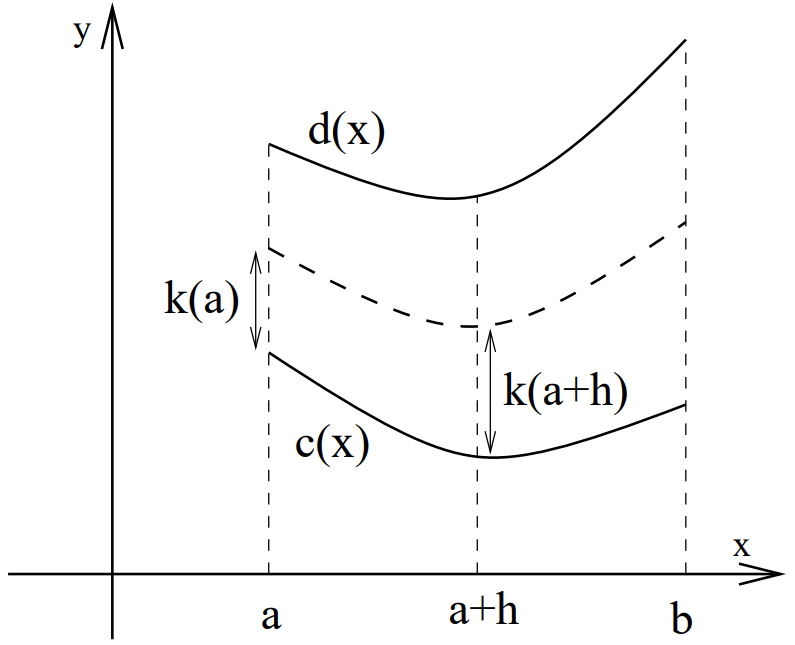
\includegraphics[width=.55\linewidth]{img/6/6_01}
		\end{figure}
        \[
        	\int_{a}^{b}\int_{c(x)}^{d(x)}f(x,\ y)dxdy;
        \]
        wzdłuż x: $h=\frac{b-a}{2}$
        $\newline$
        wzdłuż y: $k(x)=\frac{d(x)-c(x)}{2}$
\end{frame}
%%%%%%%%%%%%%%%%%%%%%%%%%%%%%%%%
\begin{frame}
	\[
    	I\approx\int_{a}^{b}\{\ \frac{k(x)}{3}[f(x,\ 
        c(x))+4f(x,\ c(x)+k(x))+f(x,\ d(x))]\}dx\approx\ldots
    \]
    \begin{block}{Zadanie}
        	Powyższy wzór - dokładniej
            $\newline$
            każda z całek - wzór Simpsona
   \end{block}
\end{frame}
%%%%%%%%%%%%%%%%%%%%%%%%%%%%%%%
\begin{frame}{Obszar regularny}
	\begin{block}{}
      \begin{itemize}
      \item całkowanie zewnętrzne - wewnętrzne
      \item dla ustalonego y - właściwy dobór x
      \item nie stosujemy regularnej siatki prostokątnej
      \end{itemize}
	\end{block}
\end{frame}
%%%%%%%%%%%%%%%%%%%%%%%%%%%%%%%%%%
\begin{frame}{Uwagi ogólne}
	\begin{enumerate}
	\item całki n-D nie są proste!
    \item złożoność obliczeniowa:
    	\begin{itemize}
    		\item 1-D $\rightarrow$ 30 obliczeń funkcji
            \item 3-D $\rightarrow$ $30^3 = 27000$ obliczeń!
    	\end{itemize}
    \item obszar całkowania:
    	\begin{itemize}
    		\item 1-D $\rightarrow$ zdefiniowany przez 2 punkty 
    	\end{itemize}
    \item n-D $\rightarrow$ $(n-1)D$ granica $\rightarrow$ skomplikowana!
	\end{enumerate}
\end{frame}
%%%%%%%%%%%%%%%%%%%%%%%%%%%%%%%%%%
\begin{frame}
	   \begin{figure}[h]
			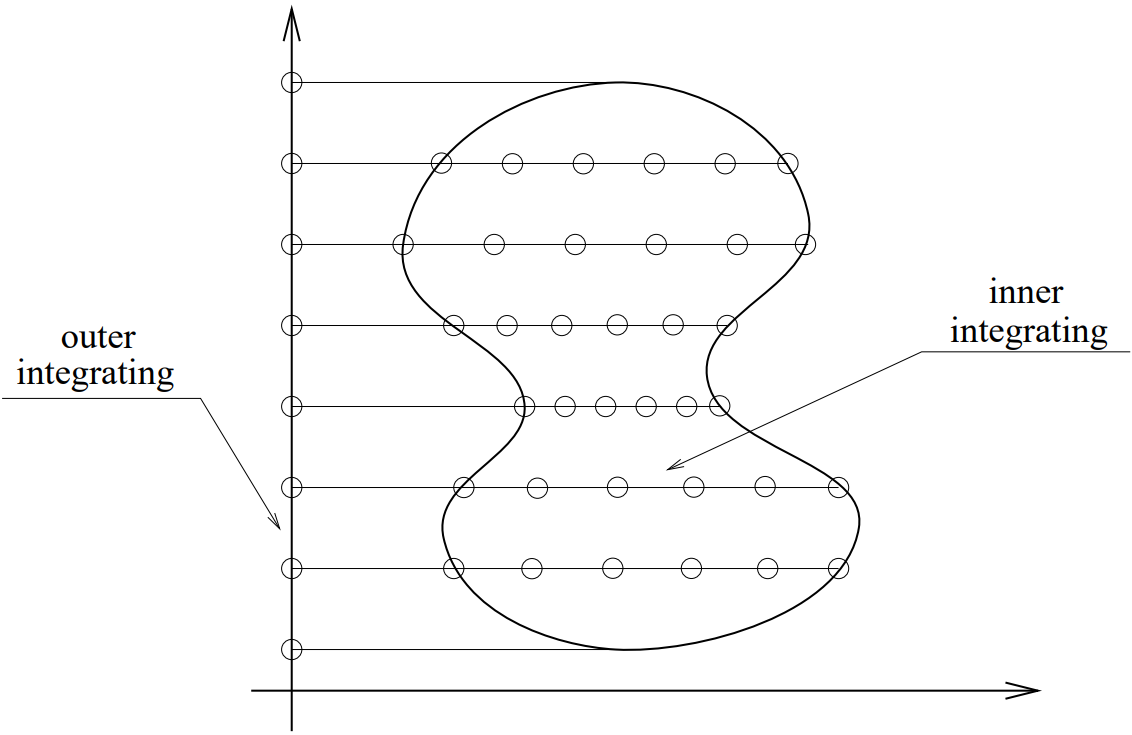
\includegraphics[width=.85\linewidth]{img/6/6_02}
		\end{figure}
\end{frame}
%%%%%%%%%%%%%%%%%%%%%%%%%%%%%%%%%
\begin{frame}
	\begin{large}
		\textbf{Podejście:}
	\end{large}
	\begin{itemize}
	\item analityczme (co się da!)
    \item wykorzystać symetrie
    \item metoda całkowania zależna od przebiegu funkcji w poszczególnych obszarach
    \item stosowanie metod Monte-Carlo
	\end{itemize}
\end{frame}
%%%%%%%%%%%%%%%%%%%%%%%%%%%%%%%%
\begin{frame}
	Całkę n-krotną można wyrazić wzorem przybliżonym:
    \[
     \int \ldots \int_{A} w(x_{1}, \ldots , x_{n})
     f(x_{1}, \ldots , x_{n})dx_{1},\ldots , dx_{n}
     \approx
     \sum_{i=1}^{n}H_{i}f(x_{1}^{(i)}, \ldots , x_{n}^{(i)})
    \]
    $A$ - obszar, $\ \ $ $w(x_{1}, \ldots , x_{n})$ - waga
    $\newline$
    $H_{i}, x^{(i)}_{j}$ - dobrane tak, by wzór był dokładny dla 
    wielomianu stopnia $\leq d$
    \begin{block}{Zadanie}
        	Wyznaczanie całek niewłaściwych
   \end{block}
\end{frame}





































	%%%%%%%%%%%%%%%%%%%%%%%

\end{document}
